% Geometric Precursor Analysis (Phase 1)
% Auto-generated from precursor diagnostics

\section{Geometric Precursor Analysis}

\subsection{Trajectory Geometry as Early-Warning Signal}

We introduce trajectory curvature $\kappa(t) = \|\boldsymbol{\eta}' \times \boldsymbol{\eta}''\| / \|\boldsymbol{\eta}'\|^3$ as a coordinate-independent early-warning signal for regime transitions. This geometric measure captures how sharply the phase-space trajectory turns in $(\eta_1, \eta_2, \eta_3)$ coordinates, independent of the basis choice.

\subsubsection{Multi-Scale Indicator Categories}

\textbf{Category A: Critical-Transition Indicators} (classical theory validation)
\begin{itemize}
    \item Multi-scale variance: $\text{Var}_\tau[\eta_3]$ for $\tau \in \{5, 15, 30, 60\}$ minutes
    \item Lag-1 autocorrelation: $\text{AC}_1^\tau(\eta_3)$ tests for critical slowing down
\end{itemize}

\textbf{Category B: Geometric Indicators} (novel in SBL context)
\begin{itemize}
    \item Trajectory speed: $v(t) = \|\mathrm{d}\boldsymbol{\eta}/\mathrm{d}t\|$
    \item Acceleration magnitude: $a(t) = \|\mathrm{d}^2\boldsymbol{\eta}/\mathrm{d}t^2\|$
    \item Trajectory curvature: $\kappa(t)$ (regularized where $v > \epsilon$)
\end{itemize}

\subsection{ FLOSS Precursor Diagnostics}

Campaign characteristics:
\begin{itemize}
    \item Duration: 11732.5 hours (488.85 days)
    \item Samples: 70796 profiles at 9.9-minute intervals
    \item State-space range: $\eta_3 \in [-80.92, 106.96]$
    \item Mean trajectory speed: $\bar{v} = n/a$
\end{itemize}

\begin{figure}[htbp]
    \centering
    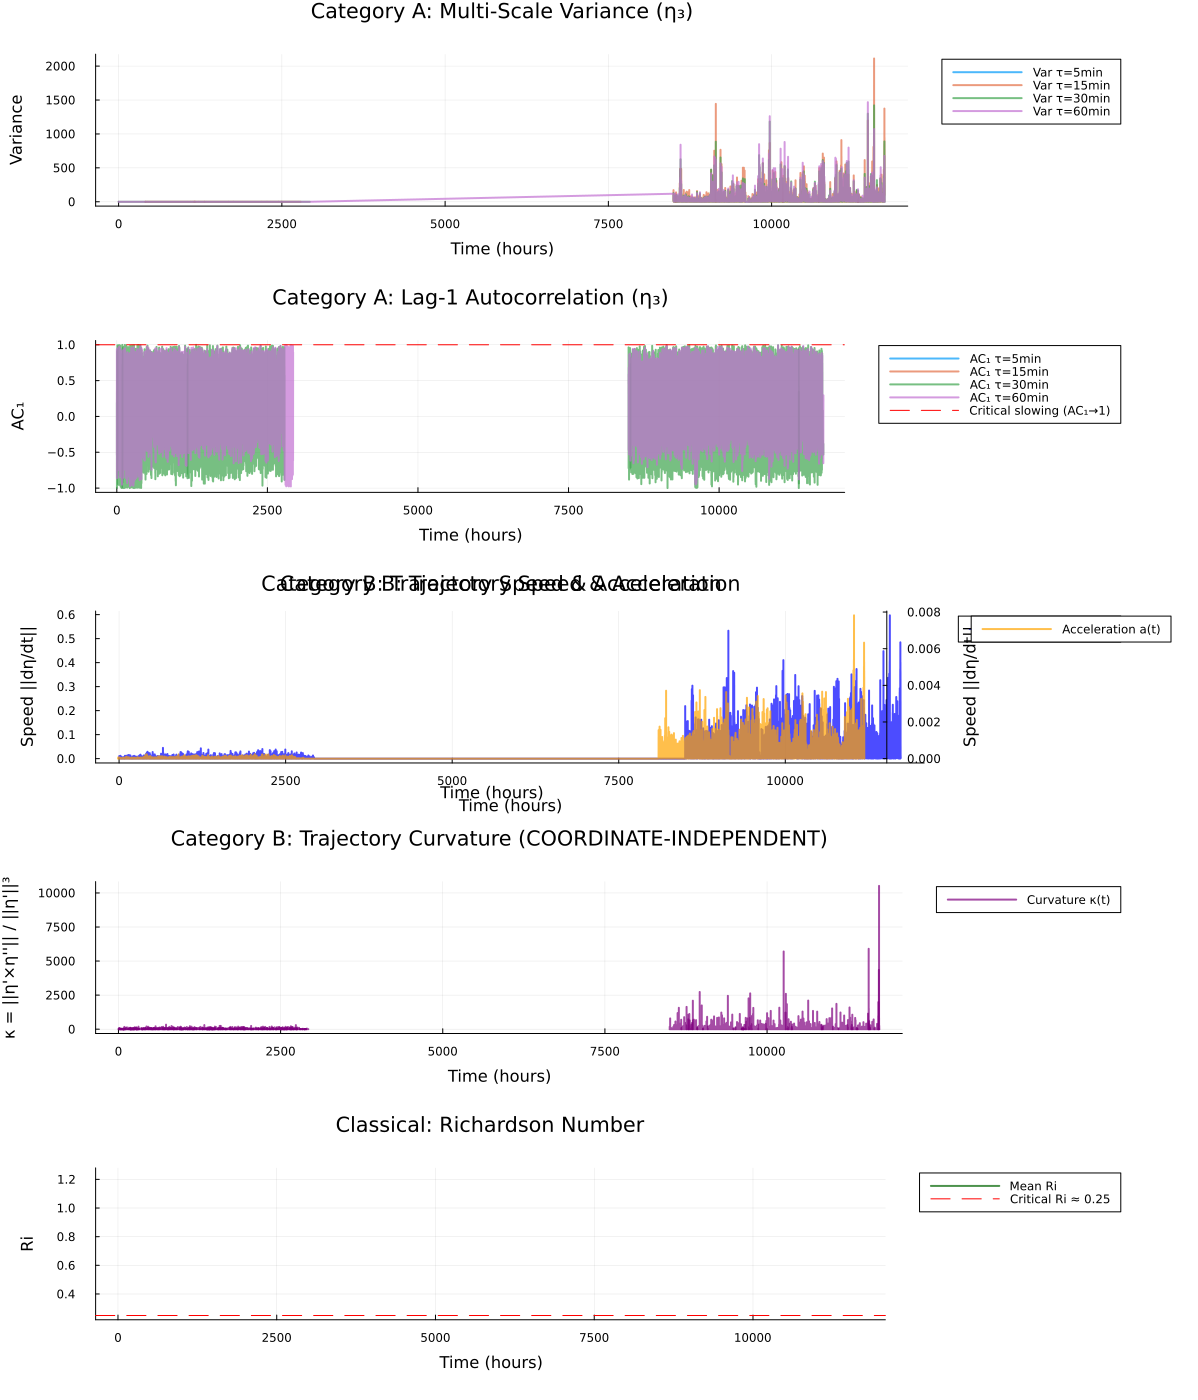
\includegraphics[width=\textwidth]{ precursor_diagnostic_floss.png }
    \caption{Multi-panel geometric precursor time series for FLOSS. 
    Panels show (top to bottom): Category A variance indicators, Category A autocorrelation, 
    Category B speed \& acceleration, Category B trajectory curvature (coordinate-independent), 
    and classical Richardson number. Vertical markers indicate identified transition events.}
    \label{fig:precursor_floss}
\end{figure}

\subsubsection{Key Observations}



\subsection{Physical Interpretation}

High curvature $\kappa \gg \bar{\kappa}$ indicates trajectory \emph{sharply turning} in manifold space---not merely moving fast (speed $v$) or changing rapidly (acceleration $a$), but undergoing rapid rotation in the direction of motion. Physically, this corresponds to:
\begin{itemize}
    \item Boundary layer restructuring events
    \item Navigation of folds in equilibrium manifold
    \item Transitions between distinct dynamical regimes
    \item Possible precursor to bifurcation (approaching/departing critical manifold regions)
\end{itemize}

